\documentclass[aps, pra, 10pt, twocolumn, superscriptaddress,floatfix]{revtex4-1}

\usepackage{amsmath,amssymb,amsfonts}
\usepackage{braket}
\usepackage[breaklinks=true,colorlinks,citecolor=blue,linkcolor=blue,urlcolor=blue]{hyperref}
\usepackage{mathtools}
\usepackage{dsfont}

%%
\def \id {\mathds{1}}
\def \abs {\text{Abs}}
\newcommand{\norm}[1]{\lVert#1\rVert}
\DeclareMathOperator{\tr}{Tr}
\newcommand{\round}[1]{\ensuremath{\lfloor#1\rceil}}
\newcommand{\mi}{\mathrm{i}} %% roman "i"
%

\begin{abstract}
	In a previous work we have been using an optical platform to test an offline metrological protocol for the estimation of a rotation angle at the Heisenberg scaling. In this notes we deal with the problem of fully characterizing the apparatus, which means estimating the current rotation angle and the visibilities of its components. In order to do so we employ a Bayesian procedure. \textbf{In the previous notes on the Bayesian procedure we repeated many times one experiment in order to estimate the mean square error (MSE). In these notes however we report the MSE computed from the internal posterior probability distribution of the Bayesian algorithm. In this way we do not have to repeat the experiment many times.}
\end{abstract}

\begin{document}
%
\title{Complete characterization of a metrological optical setup} 
%
\author{Federico Belliardo}
\email{federico.belliardo@sns.it}
\affiliation{NEST, Scuola Normale Superiore, I-56126 Pisa,~Italy}

\maketitle


\section{Introduction}
%
In this work we want to study the complete characterization of an optical setup, that might be later used by the experimentalists to carry out quantum protocols. We are going to employ the q-plate setup of~\cite{Cimini2021}, see Fig.~\ref{fig:apparatus}, with three q-plates. This means the apparatus will be characterized by four visibilities: one for the configuration without active q-plates and three for the three configurations with only one q-plate active each. 
%
\begin{figure}[!th]
	\begin{center}
		\includegraphics[width=0.5\textwidth]{FigureSetup.pdf}
	\end{center}
	\caption{View of the experimental apparatus with the three q-plates.}
	\label{fig:apparatus}
\end{figure}
%
Therefore the parameters to estimate are a rotation angle $\theta \in [0, \pi)$ and the four visibilities $V_1, V_2, V_3, V_4 \in [0, 1]$. In all the Bayesian experiments performed here the prior distributions on the visibilities will be uniform in $[0, 1]$. The Bayesian procedure will be implemented as presented in~\cite{Granade2012} with a particle filter. This method selects the next measurement to be done (the next q-plate) according to the posterior probability distribution for the unknown phase and visibilities. We will first measure only the phase $\theta$ treating the visibilities as \textit{nuisance} parameters. That means our goal will be first the minimization of the mean square error on the phase only. Here the estimators for the visibilities should be only precise enough to allow us to find a good strategy for the estimation of the phase. Then we will minimize the error on a couple of parameters, that is the phase and one of the visibilities: $(\theta, V_i)$ with $i=1, 2, 3, 4$, the other three visibilities will be again nuisance parameters. At the end we try to estimate all the five parameters $(\theta, V_1, V_2, V_3, V_4)$ at the same time. 

\section{The Bayesian procedure}
%
In this section we present the Bayesian algorithm proposed in~\cite{Granade2012}, with the application to our q-plates setup in mind. With respect to the original formulation we made a few corrections necessary because of the circular nature of the angular variable that we are going to measure. In every simulated experiment  a constant number of particles equal to $n_p = 5000$ have been used. The parameters to estimate are collected in the vector $\boldsymbol{x} := \left( \theta, V_1, V_2, V_3, V_4 \right)$, that contains the phase in the first entry and the four visibilities in the other ones. Being the Granade's method based on a particle filter, it represents internally the posterior probability distribution with the ensemble $\mathcal{E} := \lbrace \boldsymbol{x}^i, w^i \rbrace$, where $\boldsymbol{x}^i$ is the position of the $i$-th particle and $w^i$ its weight. The $j$-th component of the $i$-th particle of the ensemble will be represented as $x_j^i$, and could correspond to the phase if $j=0$, that is $x^i_0 = \theta^i$ or to one of the visibilities if $j=1, 2, 3, 4$, that is $x^i_j = V^i_j$. The mean of the angular values is computed as
%
\begin{equation}
	\hat{\mu}_0 := \arg \left[ \sum_{i=1}^{n_{p}} w^i \exp \left( \mi \theta^i \right) \right] \; ,
\end{equation}
%
while the mean values of the visibilities are
%
\begin{equation}
	\hat{\mu}_j = \sum_{i=1}^{n_p} w^i V^i_j \; .
\end{equation}
%
Together they form the vectorial mean of the distribution $\boldsymbol{\hat{\mu}} = (\hat{\mu}_0, \hat{\mu}_1, \hat{\mu}_2, \hat{\mu}_3, \hat{\mu}_4)$. The covariance matrix is defined as
%
\begin{equation}
	\text{Cov}_{ij} := \sum_{k=1}^{n_{p}} w^k (x^k_i - \hat{\mu}_i)  (x^k_j - \hat{\mu}_j) \; .
\end{equation}
%
If $i=1$ or $j=1$ then difference in $x^k_i - \hat{\mu}_i$ or $x^k_j - \hat{\mu}_j$ is actually the circular distance
%
\begin{equation}
	d(x^k_i, \hat{\mu}_i) = \pi - | (x^k_i - \hat{\mu}_i) \mod 2 \pi - \pi| \; .
\end{equation}
%
The Bayesian algorithm tries for each new experiment (each new photon sent with a specific q-plate activated) to minimize the scalar variance of the posterior distribution, that is
%
\begin{equation}
	\sigma^2 := \tr \left[ G \cdot \text{Cov} \right] = \sum_{i, j} G_{ij} \text{Cov}_{ij} \; ,
\end{equation}
%
where $G$ is the weight matrix that control which parameters are to be treated as nuisance parameters. In this way the algorithm attempts to concentrate as much as possible the distribution around its mean in a greedy fashion. In the plots of Sec.~\ref{sec:results} we reported the MSE, which is computed just like the covariance matrix but using the vector of true values $\boldsymbol{x}$ instead of the estimated mean $\boldsymbol{\hat{\mu}}$. The resampling strategy of the Granade procedure has also undergone minor changes to adapt it to the phase estimation problem. We have performed only simulations (we didn't use the actual experimental data collected) with visibilities $V_1 = 0.900$, $V_2 = 0.875$, $V_3 = 0.850$ and $V_4 = 0.765$, for $17$ angles chosen in $[0, \pi)$ that have been measured in the actual experiment. At difference with the offline algorithm we can't perform an estimation with a fixed number $N$ of total used resources, because the number of photons to use for each q-plate is a stochastic variable, that makes $N$ a stochastic variable too. Only the total number of used photons can be fixed.  In the rest of this section we will refer to the estimation of the rotation angle only, that is the MSE will be $\Delta^2 \hat{\theta}$. If two or more parameters are to be evaluated the MSE on the angle should be substituted with the sum of the errors, e.g. $\Delta^2 \hat{\theta} + \Delta^2 \hat{V}$. In order to give a synthetic representation of the performances of the Bayesian method we proceed as following. We perform an estimation for each of the angles with a total number of resources $N=30000$, and save for each new photon measurement the error $\Delta^2 \hat{\theta}$ and the total number of used resources $N$ up to that point. We plot all the points $(N, \Delta \hat{\theta})$ collected in this way for every phase in the same plot, and associate all the estimations made with a number of resources in the interval $[N, N + \Delta N]$. We compute the mean MSE of this cloud of points, that in general could refer to different angles:
%
\begin{equation}
	\overline{\Delta^2 \hat{\theta}} := \frac{1}{C} \sum_{i=1}^{C} \Delta^2 \hat{\theta}^{(i)} \; ,
\end{equation}
%
where $C$ is the number of points in the cloud and $\Delta^2 \hat{\theta}^{(i)}$ is the $i$-th point in the cloud (it can come from whatever true angle $\theta_j$). 
%
\begin{figure}[!t]
	\begin{center}
		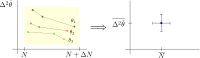
\includegraphics[width=0.5\textwidth]{cloud.pdf}
	\end{center}
	\caption{A cloud of points corresponding to different phases and different used resources (in the interval $[N, N + \Delta N]$) is substituted with a single point with average MSE and total used resources.}
	\label{fig:cloud}
\end{figure}
%
In Fig.~\ref{fig:cloud} we see an example of such procedure with only three phases and $C=9$, that means $9$ points are in the region $[N, N + \Delta N]$. On average we expect the same contribution (in terms of the number of points) from every phase. The average of the employed resources is
%
\begin{equation}
	\overline{N} := \frac{1}{C} \sum_{i=1}^C N^{(i)} \; .
\end{equation}
%
The plots of Sec.~\ref{sec:results} represent the points $(\overline{N}, \overline{\Delta^2 \hat{\theta}})$ computed for every interval $[N, N + \Delta N]$ in $[1, 30000]$. 
%The variance of the set $ \lbrace \Delta^2 \hat{\theta}^{(i)} \rbrace$ and of the resources $\lbrace N^{(i)} \rbrace$ are respectively the vertical and the horizontal error bars associated to the new points $(\overline{N}, \overline{\Delta^2 \hat{\theta}})$. 
The value of $\Delta N$ changes according to $N$, in particular we have $\Delta N = 2$ for $N \in \left[2, 100 \right]$, $N = 20$ for $N \in \left[100, 1000 \right]$ and $\Delta N = 50$ for $N \in \left[1000, 30000 \right]$. 
%\textbf{The error computed in these notes are very different from the error we gave in the precedent notes}.

\section{Bound on the precision of the joint estimation}
%
When estimating only the phase $\theta$ the most fundamental bound we can refer to is the Heisenberg limit, that dictates
%
\begin{equation}
	\Delta^2 \hat{\theta} \ge \frac{\pi^2}{N^2} \; .
	\label{eq:phaseBound}
\end{equation}
%
Regarding the estimation of the visibility, only the measurements performed with the correct q-plate switched on can contribute to it. Consider $n$ repetitions of a couple of Type-$0$ and Type-$+$ measurements~\cite{Belliardo2020}, that produce two results $c_1, c_2 \in \lbrace -1, +1 \rbrace$, extracted from the following two probability distribution
%
\begin{equation}
	p_1(c_1; \theta, V) = \frac{1 + c_1 \cdot V \cos (s \theta)}{2} \; ,
\end{equation}
%
and 
%
\begin{equation}
	p_2(c_2; \theta, V) = \frac{1 + c_2 \cdot V \sin (s \theta)}{2} \; ,
\end{equation}
%
our goal is to bound the precision on $V$. We compute the Fisher information matrix for the estimation of the couple of parameters $V$ and $\theta$ from $n$ repetition each of the Type-$0$ and Type-$+$ measurements, called respectively $n I_1 (\theta, V)$ and $n I_2(\theta, V)$, and sum them to obtain the total Fisher Information $I(\theta, V) := n I_1 (\theta, V) + n I_2 (\theta, V)$, having the inverse
%
\begin{eqnarray*}
	I^{-1} ( \theta, V) = \frac{1}{n} \begin{pmatrix}
	\frac{4 - V^2 + V^2 \cos (4 s \theta)}{4 s^2 V^2} & \frac{V \sin (4 s \theta)}{4s} \\
		\frac{V \sin (4 s \theta)}{4s} & \frac{4 - 3 V^2 - V^2 \cos (4 s \theta)}{4} \;
	\end{pmatrix}\; .
\end{eqnarray*}
%
The component $I^{-1}_{22}(\theta, V)$ of the Fisher information gives a bound on the precision of an unbiased estimator of $V$, when $\theta$ is not known, that reads
%
\begin{equation}
	\Delta \hat{V}^2 \ge \frac{4 - 3 V^2 - V^2 \cos (4 s \theta)}{4 n} \; .
\end{equation}
%
This is the minimum error for the visibilities in case the phase is not known and has to be estimated from measurements extracted according to the probability distribution $p_1(c_1; \theta, V)$ and $p_2(c_2; \theta, V)$. However the phase won't be extracted only from this measurement, rather it will be the product of an estimation involving all the q-plates with different charges. This makes the interplay between $\theta$ and $V$ in the joint estimation more complicated. The only bound we can give to the joint error $\Delta^2 \hat{\theta} + \Delta^2 \hat{V}$ is the sum of the precision bounds for the two parameters computed as if they were estimated separately with an optimal strategy and with the other parameters known. This reads
%
\begin{eqnarray*}
	&& \Delta^2 \hat{\theta} + \Delta^2 \hat{V} \ge \left( \frac{\pi}{N} \right)^2 + \frac{\left[ I_{22}(\theta, V) \right]^{-1}}{n} = \\
	&=& \left( \frac{\pi}{N} \right)^2 + \frac{1}{n} \left[ \frac{1}{-V^2 + \csc^2(s \theta)} + \frac{1}{-V^2 + \sec^2(s \theta)} \right]^{-1} \; .
\end{eqnarray*}
%
However, we will use the expression $I^{-1}_{22}(\theta, V)$, that is more treatable than $\left[ I_{22}(\theta, V) \right]^{-1}$ and doesn't differ much from it. The maximum number of experiments $n$ that can be done for the determination of the visibility $V$ are $n=\lfloor N/s \rfloor$, and the CR bound reads therefore
%
\begin{equation}
	\Delta \hat{V}^2 \ge \frac{1}{4 \lfloor \frac{N}{s} \rfloor} \left[ 4 - 3 V^2 - V^2 \cos (4 s \theta) \right] \; .
\end{equation}
%
That means the total MSE error of the phase and the visibility is bounded as
%
\begin{equation}
	\Delta^2 \hat{\theta} + \Delta^2 \hat{V} \ge \left( \frac{\pi}{N} \right)^2 +  \frac{1}{4 \lfloor \frac{N}{s} \rfloor} \left[ 4 - 3 V^2 - V^2 \cos (4 s \theta) \right] \; .
\end{equation}
%
We can take the average of this expression on the phases $\theta \in \left[0, \pi \right)$ and get
%
\begin{equation}
	\Delta^2 \hat{\theta} + \Delta^2 \hat{V} \ge \left( \frac{\pi}{N} \right)^2 +  \frac{1}{4 \lfloor \frac{N}{s} \rfloor} \left( 4 - 3 V^2 \right) \; .
\end{equation}
%
The variance of $\hat{V}$ cannot be greater than one, moreover we need to regularize the above expression for $N < s$, we write therefore
%
\begin{equation}
	\Delta^2 \hat{\theta} + \Delta^2 \hat{V} \ge \left( \frac{\pi}{N} \right)^2 + \min \Big \lbrace \frac{1}{4 \lfloor \frac{N}{s} \rfloor} \left( 4 - 3 V^2 \right), 1 \Big \rbrace \; .
\end{equation}
%
The CR bound used here applies to an unbiased estimator. We can expect the particle filter to give unbiased estimators only in the asymptotic limit, that means we cannot expect the above bound to hold rigorously for small $N$. The CR bound for a generic (biased) estimator would need the knowledge of the local behaviour of the estimator, i.e. $d \mathbb{E} [\hat{\theta}] / d \theta$, but we only have a punctual knowledge of it. We could try to massage the bound to be more adequate in the low resources region, and notice that at the beginning of the estimation the posterior probability distribution for the visibility is uniform, and therefore has mean $\mu = 0.5$ and variance $\sigma^2 = 1/12$. The RMSE is accordingly $\Delta^2 \hat{V} = \sigma^2 + (0.5 - V)^2$. It is reasonable to assume that the MSE will never be greater than this values, because as soon as the measurements begin the Bayesian algorithm seeks to reduce the variance of the posterior. We can therefore write
%
\begin{equation}
	\Delta^2 \hat{\theta} + \Delta^2 \hat{V} \ge \left( \frac{\pi}{N} \right)^2 + \min \Big \lbrace \frac{1}{4 \lfloor \frac{N}{s} \rfloor} \left( 4 - 3 V^2 \right), \frac{1}{12} + \left( 0.5-V \right)^2\Big \rbrace \; .
	\label{eq:totalBound}
\end{equation}
%
This bound is the blue line in the plots of the following section. If we consider the estimation of all the five parameters $\theta$, $V_1$, $V_2$, $V_3$, and $V_4$ together the lower bound on the precision will be
%
\begin{eqnarray*}
	&& \Delta^2 \hat{\theta} + \sum_{i=1}^{4} \Delta^2 \hat{V}_i \ge \\ && \left( \frac{\pi}{N} \right)^2 + \sum_{i=1}^{4} \min \Big \lbrace \frac{1}{4 \lfloor \frac{N}{s_i} \rfloor} \left( 4 - 3 V_i^2 \right), \frac{1}{12} + \left( 0.5-V_i \right)^2 \Big \rbrace \; .
\end{eqnarray*}
%
with $s_1 = 1$, $s_2 = 2$, $s_3 = 11$, and $s_4 = 51$. Also the bound in Eq.~\eqref{eq:phaseBound} may be violated for very small $N$.

{\color{red} We should ue a tighter bound for the phase CR bound, that is we should use the bound
%
\begin{equation}
	\frac{4-V^2+V^2 \cos(4 s \theta)}{4 s^2 V^2} \; .
\end{equation}
%
We should also conserve $\theta$ in this bound, and not average it away. It could be a problem if I use partially a frequentist and partly a Bayesian approach. I should use a Bayesian Cramer-Rao bound with a prior distribution. We might want to use the van Tree inequality for both the visibility and the phase. The yellow bounds plot in the figures are not correct. A plot with th MSE computed for multiple repetitions of the experiment shows that the MSE doesn't converge to the yellow line. Probably some measurement with the correct q-plate are done also for low $N$. This point is however still to investigate.}


\section{Results of the simulations}
\label{sec:results}
%
In this section we report the simulated MSE compared with the theoretical bound in Eq.~\eqref{eq:phaseBound} and Eq.~\eqref{eq:totalBound}. 
%
\begin{figure}[!th]
	\begin{center}
		\includegraphics[width=0.5\textwidth]{theta.pdf}
	\end{center}
	\caption{Estimation of the rotation angle in which the visibilities are considered as nuisance parameters. The weight matrix has $G_{11} = 1$ as only non-null entry.}
	\label{fig:theta}
\end{figure}
%
\begin{figure}[!t]
	\begin{center}
		\includegraphics[width=0.5\textwidth]{thetaV1.pdf}
	\end{center}
	\caption{Estimation of the rotation angle and the first visibility (all q-plates are switched off) in which the other visibilities are considered as nuisance parameters. The weight matrix has $G_{11} = 1$ and $G_{22} = 1$ as only non-null entries. The yellow line corresponds to $\frac{1}{12} + (0.5 - V_1)^2$. {\color{red} Wrong plot.}}
	\label{fig:thetaV1}
\end{figure}
%
\begin{figure}[!t]
	\begin{center}
		\includegraphics[width=0.5\textwidth]{thetaV2.pdf}
	\end{center}
	\caption{Estimation of the rotation angle and the second visibility (for the stage $s=2$) in which the other visibilities are considered as nuisance parameters. The weight matrix has $G_{11} = 1$ and $G_{33} = 1$ as only non-null entries. The yellow line corresponds to $\frac{1}{12} + (0.5 - V_2)^2$. {\color{red} Wrong plot.}}
	\label{fig:thetaV2}
\end{figure}
%
\begin{figure}[!t]
	\begin{center}
		\includegraphics[width=0.5\textwidth]{thetaV3.pdf}
	\end{center}
	\caption{Estimation of the rotation angle and the third visibility (for the stage $s=11$) in which the other visibilities are considered as nuisance parameters. The weight matrix has $G_{11} = 1$ and $G_{44} = 1$ as only non-null entries. The yellow line corresponds to $\frac{1}{12} + (0.5 - V_3)^2$. {\color{red} Wrong plot.}}
	\label{fig:thetaV3}
\end{figure}
%
\begin{figure}[!t]
	\begin{center}
		\includegraphics[width=0.5\textwidth]{thetaV4.pdf}
	\end{center}
	\caption{Estimation of the rotation angle and the forth visibility (for the stage $s=51$) in which the other visibilities are considered as nuisance parameters. The weight matrix has $G_{11} = 1$ and $G_{55} = 1$ as only non-null entries. The yellow line corresponds to $\frac{1}{12} + (0.5 - V_4)^2$.}
	\label{fig:thetaV4}
\end{figure}
%
\begin{figure}[!t]
	\begin{center}
		\includegraphics[width=0.5\textwidth]{allParameters.pdf}
	\end{center}
	\caption{Estimation of the rotation angle and all the for visibilities jointly. The weight matrix is $G = \id$.  {\color{red} Wrong plot.}}
	\label{fig:allParameters}
\end{figure}

First of all in Fig.~\ref{fig:theta} the precision estimation for the rotation angle is showed. All the visibilities are treated as nuisance parameters. In Fig.~\ref{fig:thetaV1}, \ref{fig:thetaV2}, \ref{fig:thetaV3}, \ref{fig:thetaV4} we report the precision of the estimation of two phases and a visibility. The yellow line corresponds to $\frac{1}{12} + (0.5 - V_i)^2$. The precision of all the visibilities saturates after a certain point, apart from the fourth visibility. For the third and especially the fourth visibility is very clear how the precision on $V$ is doesn't improve until a certain number of resources is reached, from that point on $s=11$ and $s=51$ starts to be used and the error diminishes. Fig.~\ref{fig:allParameters} contains the precision for the joint estimation of all the five parameters.

{\color{red} We should actually perform a simulation by repeating the estimation $100$ times instead of relying on the interior posterior representation of the system. We could look for sign of the Heisenberg scaling in the plot for the error of $\Delta^2 \hat{\theta} + \Delta^2 \hat{V}$. At the end we want to concentrate on three points: estimation of $\theta$ wit the visibilities as nuisance parameters, estimation of the CR bound of the pairs of parameters (CR bound), estimation of all the five parameters. The reason why the simulation converge to a stationary point is probably due to the bias. The variance is used to establish the next step and it is reduced, but there is a bias in the distribution that stops the MSE from decreasing further. We should try to plot the same simulations with the variance instead of the MSE.}

{\color{blue} There was a typo in the script that produced the data. So that only the fourth plot is actually correct.}

\begin{thebibliography}{100}
	
	\bibitem{Cimini2021} V Cimini \textit{et al.}, \href{http://arxiv.org/abs/2110.02908}{arXiv:2110.02908 (2021).}
	%
	
	\bibitem{Granade2012} C E Granade \textit{et al.} 2012 \href{https://doi.org/10.1088/1367-2630/14/10/103013}{New J. Phys. {\bf 14} 103013}.
	%
	
	%\bibitem{Roccia2018} E Roccia \textit{et al.}, \href{https://www.osapublishing.org/optica/abstract.cfm?uri=optica-5-10-1171}{Optica~{\bf 5}, 1171-1176 (2018).}
	%
	
	\bibitem{Belliardo2020} F Belliardo and V Giovannetti, \href{https://link.aps.org/doi/10.1103/PhysRevA.102.042613}{Phys. Rev. A~{\bf 102}, 042613}.
	%
	

	
\end{thebibliography}

\end{document}